\documentclass[12pt]{article}

\usepackage{enumitem}
\usepackage{amsmath}
\usepackage{graphicx}
\usepackage{tikz}
\usepackage{mathtools}

\title{Tech Homework \#1}
\date{2020-10-08}
\author{b08902024\\Chih-Fu Lai}

\begin{document}
\pagenumbering{gobble}
\maketitle
\newpage
\pagenumbering{arabic}

\section*{Problem 1}
\begin{enumerate}
    \item First, autonomy might be able to reduced traffic deaths caused by human errors.
    Second, combining with connectivity and some algorithms, the time spent on stop-and-go waves can be saved.
    Lastly, autonomous vehicles might save some fuel by controlling speed or with some other techniques.
    \item A concern can be some potential information security problems, which can be caused by malicious hackers.
    Another concern lies in the situation where people might rely on their wealth to gain right of ways.
    Furthermore, some drivers may not be willing to transfer from driving by themselves to autonomous cars.
    Then these uncertainty caused by human can increase the complexity of computing.
\end{enumerate}

\section*{Problem 2}
\begin{enumerate}
    \item I prefer the first definition: deaths per billion typical journeys taken.
    No matter how much distance or hours are involved in the journey, the passenger/driver usually aims for only one destination and one task.
    It's more logical for me to measure risk based on how many tasks are completed with the transportation.
    \item Most of the time, modern people tends to choose the more time-efficient way to travel in order to save time for more important activities.
    In another case, astronauts do not have choices but to take on high risks for researching purposes.
    After all, space ships are obviously the most practical vehicle when traveling in the outer space.
\end{enumerate}

\section*{Problem 3}
\begin{enumerate}
    \item (image on next page)
    \begin{figure}
        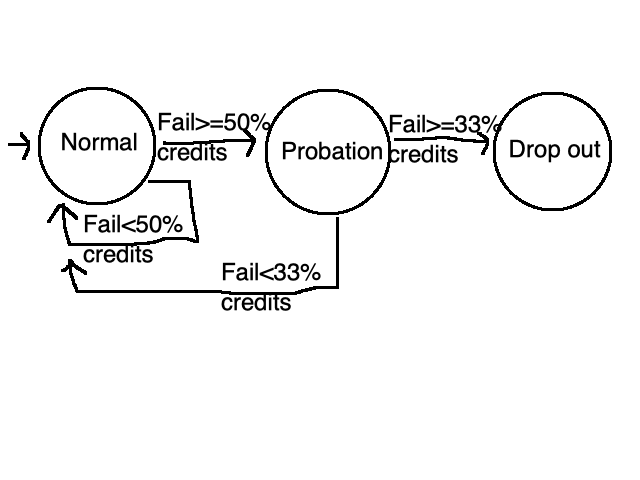
\includegraphics[width=\linewidth]{finite-state1.png}
        \label{fig:finite_state1}
    \end{figure}
    \item Student A is more likely to be dropped out. "At most once within any consecutive semesters" is actually equivalent to
    "no consecutive fails". Thus Student B can never reach the "Drop out state". On the other hand,
    It's possible for Student A to fail 33\% or more credits consecutively in some span of six years, then he might be dropped out.
    \item (image is above)
    \begin{figure}
        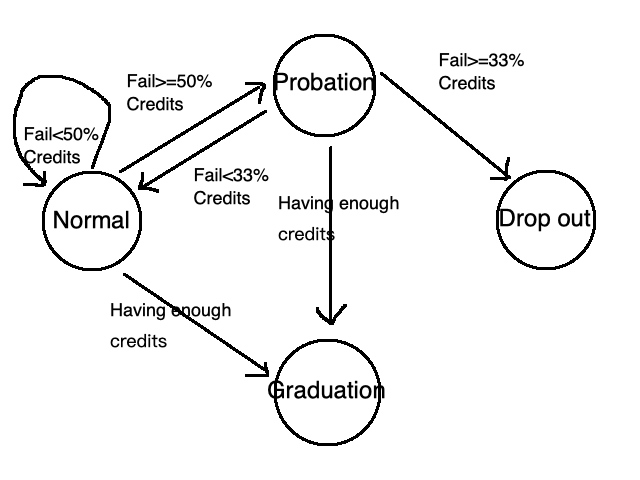
\includegraphics[width=\linewidth]{finite-state2.png}
        \label{fig:finite_state2}
    \end{figure}
\end{enumerate}

\section*{Problem 4}
\begin{enumerate}
    \item We must start from the vertex not being pointed, (1, 1), and there is a deadlock. (1, 3) needs to happen after (2, 3), but (2, 3) can never happen if (1, 3) didn't happen first in order to let (2, 1) happen.
    \item No deadlock: (2, 1), (2, 2), (1, 1), (1, 3), (2, 3).
    \item We must start from (1, 1), then the only path we can follow is (2, 1), (2, 2), (3, 2), (3, 3), (1, 3).
    However, vehicle 2 can never go to position 1 if vehicle 1 doesn't move from position 1 to 3.
    Thus, there is a deadlock.
\end{enumerate}

\end{document}